\chapter{Deseño}
\label{ch:desenho}

Neste capítulo falaremos sobre o deseño dos distintos compoñentes do sistema.
Para iso, vaise dividir en tres seccións:
\begin{itemize}
  \item Nunha primeira sección, analizaremos o modelo de datos, é dicir, as
  distintas clases que o sistema emprega para manter o estado dos distintos
  mundos de xogo.
  \item A segunda sección irá destinada a todo o relativo á linguaxe COE e o
  código ofrecido por ANTLR, e analizarase especialmente a implementación do
  patrón Visitor, crucial para a análise semántica da linguaxe.
  \item Finalmente, a terceira sección estará dedicada a DemiurgoWeb, a forma de
  funcionar de Spring en xeral e o deseño da web.
\end{itemize}

\section{Modelo de datos}
O modelo dentro do patrón modelo-vista-controlador é a parte do código
que fai referencia aos distintos datos que o programa manexa. No caso do
Demiurgo podemos atopalo nas clases contidas en dous paquetes: \textit{Universe}
e \textit{Values}.
\par
En Universe podemos atopar todas as clases relacionadas cos distintos conceptos
manexados nun mundo de xogo: \textbf{Action, ClassMethod, DemiurgoClass,
DemiurgoLocation, DemiurgoObject, DemiurgoRoom, Inventory, RoomPath,
RootObjectClass, User, Witness e World}. Máis adiante explicarase en detalle o
funcionamento de cada un deles.
\par
En Values están todas as clases que fan referencia a distintos valores que pode
conter unha variable no xogo. Todas estas clases implementan unha interface
chamada \textbf{ValueInterface}, que é a empregada no patrón Visitor como tipo a
devolver por cada visita (explicarase isto na subsección \ref{subsec:visitor}).
Estas clases son: \textbf{FloatValue, IntegerValue, ListValue, StringValue,
LocationValue, RoomValue, InventoryValue, ObjectValue}.

\begin{figure}
\centerline{\includegraphics{figuras/diagramas/clases/clases.1}}
\caption{Diagrama de clases do paquete Universe (relacións entre clases).}
\label{fig:universe}
\end{figure}

\subsection{World}
\begin{figure}
\centerline{\includegraphics{figuras/diagramas/clases/world.1}}
\caption{Clase World.}
\label{fig:world}
\end{figure}
A clase que representa un mundo de xogo concreto. Existe un obxecto de clase
World por cada partida que aloxe o Demiurgo. Esta clase contén as referencias a
todos os obxectos, clases e escenarios do mundo, así como unha lista dos
usuarios na partida. Todos estes elementos están debidamente referenciados
en \textit{maps} diferenciados, identificados polo seu identificador
correspondente (un número na maioría dos casos, un nome nos usuarios).
\par
Ademais de manter referencias, o obxecto World ofrece métodos útiles para
xestionar as relacións entre os distintos compoñentes do mundo, como un método
\textit{setObjectUser} para asignar usuarios a obxectos.

\subsubsection{RoomPath}
RoomPath é unha clase que ten como finalidade organizar os escenarios do xogo
segundo o seu nome ou ruta. A clase RoomPath emprega unha variante do patrón
\textbf{Composite}: cada RoomPath contén unha lista de fillos, e un ou ningún
escenario asociado (ver figura \ref{fig:roompath}). Deste modo, almacenando un
obxecto raíz equivalente ao escenario \textit{/}, despregando os fillos deste
obxecto atoparemos a árbore de escenarios. O funcionamento por tanto é moi
semellante ao dunha árbore de directorios.
\begin{figure}
\centerline{\includegraphics{figuras/diagramas/roompath.pdf}}
\caption{Exemplo de estrutura de escenarios. As caixas azuis representan
obxectos RoomPath, e os círculos laranxas obxectos DemiurgoRoom.}
\label{fig:roompath}
\end{figure}

\subsection{DemiurgoObject}
A clase DemiurgoObject emprégase para os distintos obxectos do xogo, entendendo
por \textit{obxecto} a definición de xogo (non un obxecto de Java). Todos os
obxectos conteñen un identificador (un número de tipo \textit{long}) e unha
lista de campos de tipo ValueInterface indexada por nome. A maiores, a clase
DemiurgoObject ten referencias á \textit{clase} (entendida segundo a definición
de xogo) do obxecto en cuestión, a súa localización (un escenario ou un
inventario) e o usuario relacionado con el en caso de ter algún.

\subsection{DemiurgoClass}
A clase DemiurgoClass fai referencia ás clases do xogo (no sentido da súa
definición de xogo). Cada clase contén un nome, unha lista de campos (indexada
por nome) e unha referencia á clase pai. Tamén conteñen unha lista de métodos.

\subsubsection{ClassMethod}
Os métodos de clase son fragmentos de código asociados a unha clase concreta cun
nome determinado. Todo método dispón dunha lista de 0 ou máis argumentos (que
son obxectos tipo ValueInterface), dos cales 0 ou máis son de saída e 0 ou 1 de
entrada. Ademais disto, contén un obxecto de tipo NodeTree (propio da libraría
ANTLR) que contén o código do método.
\par
A clase ClassMethod é filla de DemiurgoMethod, unha clase abstracta que fai
referencia a calquera tipo de método que poida ser executado no Demiurgo (tanto
métodos de clases como funcións internas).

\subsubsection{RootObjectClass}
RootObjectClass é unha clase especial que herda de DemiurgoClass. Fai referencia
á clase \textit{Object} do mundo de xogo, é dicir, a clase raíz da que herdan
todas as clases.

\subsection{DemiurgoLocation}
DemiurgoLocation é unha clase abstracta que fai referencia a calquera
localización capaz de conter obxectos. As dúas clases fillas que herdan desta
son por tanto DemiurgoRoom (escenarios) e Inventory (inventarios). Teñen en
común a posesión da lista de obxectos que ``conteñen''.
\par
As localizacións dispoñen de dous métodos útiles para o uso de inventarios: un é
\textit{isInsideOf(DemiurgoLocation)}, que devolve \textit{false} no caso dos
escenarios, pero nos inventarios devolve \textit{true} se o obxecto que o contén
se atopa dentro da localización especificada. O outro método é
\textit{getRealLocation()}, moi relacionado co anterior; se é invocado por un
escenario devolverá o propio obxecto, pero se é invocado por un inventario,
chamará ao método getRealLocation() da localización do obxecto que o contén.

\subsection{DemiurgoRoom}
DemiurgoRoom é a clase que representa un escenario no mundo. Herda de
DemiurgoLocation e contén o seu nome de escenario completo (ou \textit{ruta}),
unha lista de variables de escenario (de tipo ValueInterface) e a
\textit{``prenarración''} do escenario (é dicir, o texto obtido mediante
\textit{echos} antes de redactar a narración definitiva; máis información no
manual no apéndice \ref{ch:manual}).

\subsection{Inventory}
O inventario é unha localización especial vinculada a un campo dun obxecto
concreto. Os inventarios créanse automaticamente cando se crean obxectos que
conteñen campos de tipo ``inventario'', e destrúense cando o obxecto é
destruído (ou cando perde dito campo debido a unha modificación posterior da
clase). Herda de DemiurgoLocation e a maiores ten unha referencia ao obxecto que
o contén, así como o nome do campo asociado.

\subsection{User}
A clase User contén a información dun usuario: nome, enderezo email, decisión
actual (unha cadea de texto ou \textit{null}), e o seu rol. O seu contrasinal
non se almacena no programa, polo que será necesario acceder á base de datos
para realizar a operación de \textit{login}.

\subsubsection{UserRole}
UserRole é unha enumeración que acepta dous valores: \textit{GM} e
\textit{USER}. GM é o rol dos directores de xogo, mentres que USER é o rol dos
xogadores comúns.

\subsection{Action}
Action contén toda a información necesaria dunha acción no mundo de xogo.
Ten un identificador numérico (de tipo \textit{long}), está asociada a un
escenario concreto, e garda a narración da acción, a data e un booleano
indicando se a acción está publicada ou non.

\subsubsection{Witness}
Cada acción garda unha lista de \textit{testemuñas}, que basicamente son os
usuarios que se atopaban no escenario no momento da acción. Cada testemuña
contén o usuario en cuestión, e a \textit{decisión} do usuario nesa acción.

\subsection{Valores}
A maiores do paquete Universe, tamén convén resaltar o paquete Values, que
contén clases que fan referencia aos diferentes tipos de datos que manexa
Demiurgo. Cada clase deste paquete ten definidas as diferentes operacións que
pode realizar o seu tipo correspondente. Todas estas clases implementan a
interface ValueInterface e herdan da clase abstracta AbstractValue, que ofrece
operacións por defecto (polo xeral devolver unha excepción de tipo
\textit{IllegalOperationException}). Os valores teñen asignado un valor da
enumeración \textit{ReturnValueTypes} que identifica o tipo de valor.
\subsubsection{Valores primitivos}
As clases IntegerValue, FloatValue e StringValue representan os valores
primitivos de números enteiros, flotantes e cadeas de texto. O seu contido está
asociado ao obxecto ValueInterface correspondente, polo que ao usalo como
argumento pásase por valor (non por referencia).
\subsubsection{ListValue}
A clase ListValue representa listas de outros elementos. Ademais de gardar o seu
tipo (``LIST''), almacena un tipo diferente chamado \textit{innerType}, que fai
referencia ao tipo de elementos que contén. Tamén garda a profundidade da lista
(\textit{depth}). Estes dous valores son necesarios para definir totalmente o
tipo dunha lista: non se pode asignar unha lista a unha variable lista con tipos
internos diferentes ou con profundidades distinta.
\subsubsection{ObjectValue}
Contén unha referencia a un obxecto concreto. Dous ou máis obxectos ObjectValue
poden facer referencia ao mesmo obxecto.
\subsubsection{RoomValue}
Clase filla de LocationValue, contén unha referencia a un escenario.
\subsubsection{InventoryValue}
Clase filla de LocationValue, contén unha referencia a un inventario. A
diferencia de RoomValue, non pode xerarse de forma normal no código, nin
enviarse como argumento; tampouco pode asignárselle un valor distinto ao que xa
posúe. Isto é para evitar que os campos de inventario dun obxecto poidan ser
reasignados e se perda a referencia orixinal ao inventario orixinal. 


\section{Deseño da linguaxe COE}
Como xa se explicou en capítulos anteriores, o intérprete da linguaxe COE foi
desenvolvido empregando o software ANTLR, un programa deseñado para ler
gramáticas e xerar analizadores léxico-sintácticos a partir delas. Por tanto, o
primeiro paso necesario para a elaboración deste intérprete foi unha definición
formal da gramática de forma que ANTLR puidera entendela, mediante un ficheiro
.g4.

\subsection{Gramática}
O ficheiro coa gramática pode atoparse no código fonte, na ubicación
/src/main/antlr/COE.g4 (seguindo a estrutura propia de Maven). O ficheiro está
composto por unha serie de regras, que como podemos ver no manual de
ANTLR\cite{antlr4} teñen a seguinte forma:
\begin{lstlisting}
nomeDaRegra : <<alternativa1>> | ... | <<alternativaN>> ;
\end{lstlisting}
\par
As alternativas, á súa vez, poden tratarse de outras regras ou de tokens léxicos
(tales como números ou cadeas de texto concretas), os cales están definidos ao
final do ficheiro; distínguense polo feito de ter as regras o nome en
maiúsculas. Deste modo, a partir da gramática, o analizador léxico-sintáctico
xerado por ANTLR pode analizar calquera código introducido e devolver unha
árbore sintáctica segundo as regras definidas, ou devolver unha excepción se o
código non ten equivalencia posible; implicando este caso que o código é
incorrecto.
\par
No caso da gramática de COE, a regra \textit{``s''} é a regra inicial pola que
comeza o proceso de análise. O primeiro que se pode observar é que ofrece dúas
alternativas (se non temos en conta o texto baleiro): definición de clase, ou
código. O primeiro caso implica definir unha nova clase para o mundo, mentres
que o segundo correspóndese coa execución de código nun escenario concreto.
Estas dúas regras por tanto correspóndense con dous contextos distintos do
programa; no caso de empregalos incorrectamente (por exemplo, introducindo
código corrente no canto dunha definición de clase) o sistema devolverá un erro;
non obstante, iso definirase na análise semántica, e resulta irrelevante á hora
de crear a árbore sintáctica.
\par
No caso da definición de clase, a regra determina unha sintaxe concreta que
permite definir nome da clase, clase pai, os distintos campos e os métodos; cabe
destacar que a regra que define un método concreto contén a regra do código
corrente, polo se un input de código determindo é aceptado nunha acción nun
escenario, tamén será aceptado nun método dunha clase polo analizador
sintáctico.
\par
No caso do código dunha acción, este está composto por regras chamadas
\textit{``line''}, é dicir, liñas de código. Cada unha destas liñas pode ser:
\begin{itemize}
  \item Unha operación,
  \item Unha expresión condicional ``if'',
  \item Un bucle ``for'',
  \item Unha asignación de obxecto a un usuario,
  \item Unha declaración dunha variable,
  \item Un \textit{echo} (output de texto).
\end{itemize}
\par
Á súa vez, as operacións poden conter outras operacións, o que permite
combinalas tal e como indica o manual (apéndice \ref{ch:manual}).

\subsection{Proceso de análise}
ANTLR xera código na linguaxe que especifiquemos (que neste caso será Java) que
permite facer a análise léxica e sintáctica do código, polo que aforramos ter
que implementar ese compoñente pola nosa parte. O que nos ofrece ANTLR son
clases que permiten enviar como argumento un InputStream co código a analizar e
devolven unha árbore sintáctica.
\par
Cando executamos ANTLR coa gramática COE, devolve os seguintes ficheiros:
\begin{itemize}
  \item COE.tokens: Non é unha clase Java. Recopila todos os tokens definidos
  na gramática e asigna un identificador único a cada un deles.
  \item COELexer: Analizador léxico. Le o código como texto e ``esnaquízao'' en
  tokens para que o analizador sintáctico poida lelos.
  \item COEParser: Analizador sintáctico. Analiza o fluxo de tokens producido
  polo analizador léxico e organízaos nunha árbore sintáctica segundo definan as
  regras da linguaxe.
\end{itemize}
\par
Unha vez estamos neste punto, o seguinte será percorrer a árbore sintáctica e
executar realmente o código, é dicir, interpretar o significado das distintas
regras e realizar as mudanzas correspondentes no mundo de xogo. Este paso
coñécese como \textbf{análise semántica}, e ANTLR ofrece dúas formas de
realizalo:
\begin{itemize}
  \item Listener: Por defecto ANTLR xera unha clase que implementa o patrón
  \textit{Listener}, que é quen de percorrer unha árbore sintáctica e producir
  eventos cada vez que entra ou sae dunha norma. É unha forma sinxela de
  realizar a análise semántica, pero non nos ofrece o control do fluxo que
  precisamos para unha linguaxe como a linguaxe COE, polo que non o
  empregaremos.
  \item Visitor: É posible especificar que ANTLR xere unha clase que implemente
  o patrón \textit{Visitor} para percorrer a árbore. Esta é a solución que
  escollimos neste proxecto, e será explicado na subsección
  \ref{subsec:visitor}.
\end{itemize}

\subsection{Patrón Visitor}
\label{subsec:visitor}
Para evitar a pesadez de ter que implementar manualmente unha clase que percorra
a árbore sintáctica e a interprete debidamente, ANTLR ofrécenos a posibilidade
de definir unha clase que implemente o patrón Visitor a partir dunha interface
que xera xunto cos analizadores léxico e sintáctico. O patrón explícase
brevemente no manual de ANTLR \cite{antlr4}; pódese ver un diagrama na figura
\ref{fig:visitor}.

\begin{figure}
\centerline{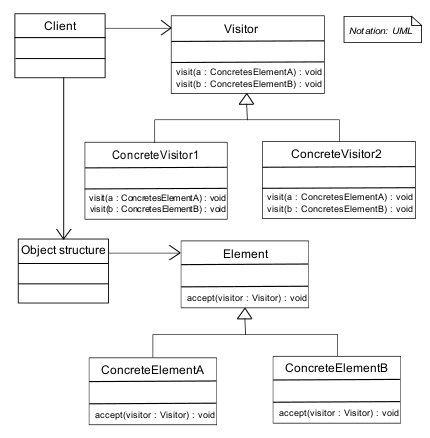
\includegraphics{figuras/diagramas/visitor.png}}
\caption{Diagrama de clases xenéricodo patrón Visitor.}
\label{fig:visitor}
\end{figure}

\begin{figure}
\centerline{\includegraphics{figuras/diagramas/coevisitor.pdf}}
\caption{Diagrama de clases do patrón Visitor aplicado no proxecto.}
\label{fig:coevisitor}
\end{figure}

\par
O funcionamento resumido pódese ver no diagrama da figura \ref{fig:coevisitor}:
ANTLR xera unha interface chamada COEVisitor, a cal debemos implementar para
xerar o noso propio Visitor (CodeVisitor neste caso). A interface danos un
método ``visit'' por cada regra que atope na gramática. Neste caso, por
simplificar, teremos en conta só dúas entradas: Code, relativo á regra chamada
\textit{code}, e SCode, relativo á segunda alternativa da regra chamada
\textit{s} (isto é, a que seguiría no caso de atopar código), tal e como o
definimos na gramática:
\begin{lstlisting}
s : nl? class_def nl?   #classDef
    | nl? code nl?      #sCode
    |                   #empty
    ;
\end{lstlisting}
Por tanto, a interface ofrécenos un método chamado visitSCode(), e outro chamado
visitCode(); ambos reciben un ParseTree como argumento, unha clase que usa ANTLR
para referirse a calquera elemento da árbore sintáctica (incluída a raíz).
\par
Cabe destacar que na práctica non implementamos directamente a interface
COEVisitor, senón que ANTLR nos ofrece a maiores unha clase abstracta chamada
COEBaseVisitor da que podemos herdar que aporta métodos útiles; entre eles, o
propio método visit() que no diagrama aparece definido en COEVisitor. Este tipo
de detalles elimináronse do diagrama para simplificar o proceso.
\par
Partimos da base de que a execución do analizador léxico e sintáctico
nun código determindo devolveunos unha árbore sintáctica; isto é, un obxecto que
implementa a interface ParseTree e que contén fillos segundo estea definido nas
regras da gramática. Na realidade este nodo é un obxecto da clase
ParserRuleContext, tal e como mostra o diagrama. Entón, o proceso a seguir é
chamar ao método \textit{visit()} do novo Visitor personalizado, enviando a nosa
árbore sintáctica como argumento. Este executará o método visit() por defecto,
que non fai outra cousa máis que invocar o método \textit{accept()} do nodo
raíz.
\par
No nodo raíz, que é un obxecto de tipo SCodeContext (xa que é regra inicial da
gramática), execútase o método accept(). Tal e como describe o diagrama, este
método invoca o método \textit{visitSCode()} do Visitor, que estará definido
por nós e por tanto fará o que nós especifiquemos. A maiores, o obxecto
SCodeContext envíase como argumento e, tal e como o seu nome indica, servirá de
contexto dentro do método visitSCode(): poderemos empregar os métodos que nos
ofrece para obter os seus fillos. Neste caso, só dispoñemos do método
\textit{code()}, que nos devolve a súa regra filla chamada ``code''. Polo que
nalgún momento na definición de visitSCode(), será preciso facer
visit(ctx.code()) para seguir co proceso.
\par
Por tanto, para aplicar o patrón Visitor en ANTLR, o único que precisamos é
definir os distintos visitX() que precisemos a partir da interface no noso
Visitor personalizado.

\subsubsection{CodeVisitor e ClassVisitor}
Debido a que hai dous contextos diferenciados na execución de código no
Demiurgo (código de acción e definición de clases), implementáronse tres clases
coa interface COEVisitor:
\begin{itemize}
  \item ExecVisitor: Clase abstracta. Contén código común a ambos contextos.
  \item CodeVisitor: Filla de ExecVisitor. Contén código exclusivo do contexto
  da execución de código de acción. Almacena unha referencia ao escenario
  actual, e devolve unha excepción se recoñece código de definición de clases.
  \item ClassVisitor: Filla de ExecVisitor. Contén código específico para
  definir clases, e garda unha referencia á clase que está sendo definida. Se
  recoñece código de acción, devolve unha excepción.
\end{itemize}

\subsubsection{Scopes e ScopeManager}
Nun momento dado da execución, o \textit{scope} ou ámbito determina os símbolos
aos que ten acceso o analizador. Xunto cos Visitors implementouse un xestor de
scopes (\textit{ScopeManager}) que contén o scope que se está empregando en cada
momento, así como unha pila de scopes na que se van engadindo os scopes novos.
Podemos distinguir os seguintes (todos son clases que herdan da clase abstracta
\textit{Scope}):
\begin{itemize}
  \item WorldScope: Tamén chamado Scope global. Contén unha referencia ao mundo
  de xogo.
  \item RoomScope: O scope inicial do código de accións. Contén unha referencia
  ao escenario actual. Cando se lle solicitan símbolos, devolve variables do
  escenario.
  \item ClassScope: O scope inicial da definición de clases. Contén unha
  referencia á clase en definición. Cando se lle solicitan símbolos, devolve os
  campos da clase.
  \item ObjectScope: Este scope só se emprega en solitario cando se xeran os
  valores por defecto dun obxecto. Aparte diso, emprégase como pai de
  FunctionScope ao invocar o método dun obxecto. Contén unha referencia ao
  obxecto en cuestión, e as referencias a símbolos devolven campos do obxecto.
  \item MethodDefiningScope: Scope que é utilizado ao definir os métodos dunha
  clase. Contén os argumentos do método (que se extraerán unha vez remate a
  definición para formar o método en si), e ten unha referencia a un ClassScope
  como pai para acceder aos campos da clase en definición.
  \item LoopScope: Scope empregado nun bucle ou nun condicional. Contén unha
  lista de variables locais que desaparecen unha vez o bucle ou condicional
  rematan. Tamén ten unha referencia ao scope anterior (pai).
  \item FunctionScope: Clase filla de LoopScope empregada para os bucles for.
  Contén unha lista de valores a empregar para facer o bucle, e o nome da
  variable que empregará para almacenalos iterativamente.
  \item ForScope
\end{itemize}

\subsubsection{Xestión de erros}
ANTLR por defecto ofrece unha estratexia de xestión de erros que busca evitar
que a análise se deteña; é dicir, en caso de atopar un erro léxico ou
sintáctico, ANTLR intenta recuperarse para proseguir coa análise.
\par
Este sistema non nos serve para o proxecto, xa que a nosa pretensión é que o
sistema se deteña e mostre un erro en canto atope un erro no código, mostrando a
posición do mesmo. Debido a isto, foi necesario configurar tanto o analizador
léxico como o semántico para que empreguen a estratexia BailErrorStrategy,
definida por ANTLR, que detén a análise ante calquera erro.
\par
A maiores, foi preciso buscar o modo de deter a análise semántica en canto se
detecte un problema (por exemplo, unha operación ilegal). Para isto optouse por
encapsular as distintas excepcións que o noso Visitor pode lanzar dentro de
RuntimeExceptions, para así deter o percorrido do Visitor e poder recuperar as
causas do erro.

\section{DemiurgoWeb}